\documentclass[11pt]{scrartcl}
\usepackage{graphicx}
\graphicspath{{./}}
\usepackage[sexy]{evan}
\usepackage[normalem]{ulem}
\usepackage{hyperref}
\usepackage{mathtools}
\hypersetup{
    colorlinks=true,
    linkcolor=blue,
    filecolor=magenta,      
    urlcolor=cyan,
    pdfpagemode=FullScreen,
    }
\usepackage[most]{tcolorbox}
\renewcommand{\dangle}{\measuredangle}

\renewcommand{\baselinestretch}{1.5}

\addtolength{\oddsidemargin}{-0.4in}
\addtolength{\evensidemargin}{-0.4in}
\addtolength{\textwidth}{0.8in}
% \addtolength{\topmargin}{-0.2in}
% \addtolength{\textheight}{1in} 


\setlength{\parindent}{0pt}

\usepackage{pgfplots}
\pgfplotsset{compat=1.15}
\usepackage{mathrsfs}
\usetikzlibrary{arrows}

\title{2024 Asia International Mathematical Olympiad Open Trial Simulation 1}
\author{Question Paper}
\date{17.00, 24 April 2024 - 23.59, 26 April 2024}

\begin{document}
\maketitle
\begin{center}
    \Huge
    \boxed{\textbf{Grade 3 - 4}}
\end{center}
\vspace{3cm}

\begin{flushright}
    \huge
   Time allowed: 90 minutes
\end{flushright}

\vspace{3cm}
\normalsize
Write down the answer according to the instruction given in questions. \textbf{The calculation result are guaranteed in the integers form.} If the answer is in surd form, represent the answer which is in the simplest form. \textbf{No need to write down any unit.}

\vspace{2cm}
Link to submit the answers: \url{https://forms.gle/txbZd1f1EbCLpbe26}

\pagestyle{plain}
\newpage
Section A – each question carries 4 marks

\hrulefill %linefill

\begin{enumerate}
    \item How many two-digit prime numbers with repeated digits are there?

    \item \vspace{10cm} 12 bottles of milk contain 4 litres of milk. How many litres of milk do 45 bottles of milk contain?

    \newpage

    \item \vspace{10cm} How many terms are there in the arithmetic sequence '4, 7, 10, \ldots, 58, 61'?

    \item \vspace{10cm} Fritzy had some dumpling. After he ate 2 less than a half of the dumpling, 42 dumpling were left. How many dumpling did Fritzy have at the beginning?

    \newpage

    \item \vspace{10cm} Calculate the following expression.
    $$11 \times 13 - 17 \div 7 - 13 \times 8 +24 \div 7.$$

    \item \vspace{10cm} There are 3 red, 4 yellow, 5 blue and 6 green marbles in a bag. At least how many marbles have to be picked up to ensure that 3 marbles of different colours are picked up?

    \newpage

    \item \vspace{10cm} The sides of each small grey square are 3 centimetres long in the following figure. How many centimetres is the perimeter of the shaded area?
    \begin{figure}[h]
        \centering
        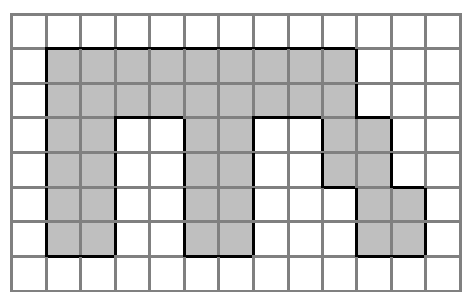
\includegraphics[width=0.4\textwidth]{StarGen/AIMO Trial G3-4 2024/perimeter-weird.png}
    \end{figure}

    \item \vspace{10cm} Find the remainder when $2763497219$ is divided by 9.

    \newpage
\end{enumerate}
\vspace{10cm}

\newpage
Section B – each question carries 5 marks

\hrulefill %linefill
\begin{enumerate}[resume]
    \item Find the value of the following expression.
    $$(1-101) \times (3-99) \times (5-97) \times (7-95) \times \ldots \times (97-5) \times (99-3) \times (101-1).$$
    
    \item \vspace{10cm} A basketball team has five players with an average height of 185 centimetres. The average height of a point guard, shooting guard and small forward is 176 centimetres. The average height of a small forward, power forward and centre is 193 centimetres. How many centimetres high is the small forward in this basketball team?

    \newpage

    \item \vspace{10cm} It is known that the 6 apple and 8 breads cost 96 dollars in total. 1 bread is 1 dollar more expensive than 2 apple. How much does 1 apple cost in dollars?

    \item \vspace{10cm} Find the value of the following expression.
    $$214+208+202+\dots+16+10.$$

    \newpage

    \item \vspace{10cm} Among the four-digit numbers which are divisible by 12 and 18, and have non-repeated digits, what is the biggest?

    \item \vspace{10cm} If a rectangle which is 3 centimetres long and 2 centimetres wide and a rectangle which is 2 centimetres long and 3 centimetres wide are treated as the same rectangle, how many kinds of rectangles with an area of 72 square centimetres whose length and width are both integers in centimetres are there?

    \newpage

    \item \vspace{10cm} Among the 2023 natural numbers from 1 to 2024, at least how many numbers have to be picked at random so that there must be two numbers whose sum is 2024?

    \item \vspace{10cm} A 7-digit number $\overline{A1234A4}$ is divisible by 12. find the sum of possibilites of $A$.

    \newpage
\end{enumerate}
\vspace{10cm}
\newpage
Section C – each question carries 7 marks

\hrulefill %linefill
\begin{enumerate}[resume]
    \item In following figure, all the angles given in the following figure are straight angles. Find the area of the figure.
    \begin{figure}[h]
        \centering
        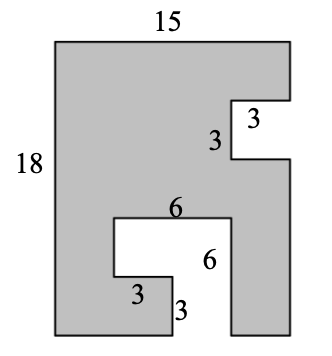
\includegraphics[width=0.4\textwidth]{StarGen/AIMO Trial G3-4 2024/nazi-area.png}
    \end{figure}
    
    \item \vspace{10cm} What is the 1000th term in the sequence '1, 1, 2, 1, 2, 3, 1, 2, 3, 4, 1, \ldots'?

    \newpage

    \item \vspace{10cm} A spider has 8 legs but no wings; A dragonfly 6 legs and 2 pairs of wings; A Cicadas 6 legs and 1 pair of wings. Now there are 27 insects of these three kinds. They have 180 legs and 25 pairs of wings in total. How many cicadas are there?
    
    \item \vspace{10cm} There is a book with 359 pages. Each page has a page number: 1, 2, 3, \ldots, 358, 359. How many ‘3’s are used in total for the page numbers of this book? 
\end{enumerate}

\end{document}